\section{Osnovni statistični pojmi}

Na kratko predstavimo statistične pojme, ki jih moramo razumeti za nadaljna poglavja. Definicije niso formalne, saj je namen tega poglavja bralcu razumljivo predstaviti te pojme na enostaven in pregleden način. Bralec, ki dobro pozna osnovne pojme statistike in teorije verjetnosti, lahko to poglavje izpusti.

Začnimo z definicijami osnovnih statističnih pojmov:

\begin{definicija}
	\leavevmode
	\begin{enumerate}
		\item \textbf{Statistična populacija} (ali \textbf{populacija}) je množica vseh proučevanih elementov. Potrebna je natančna časovna in krajevna opredelitev.
		\item Dovolj velika podmnožica populacije, tj. podmnožica, na osnovi katere lahko sklepamo lastnosti celotne populacije, imenujemo \textbf{vzorec}.
		\item Posameznemu proučevanemu elementu populacije/vzorca pravimo \textbf{enota}.
		\item \textbf{Spremenljivka} je lastnost enot.
	\end{enumerate}
\end{definicija}

Poglejmo si primer statistične populacije:

\begin{zgled}
	Vzemimo populacijo vseh študentov v 2. letniku matematike na Fakulteti za matematiko in fiziko (krajevna opredelitev) v šolskem letu 2018/2019 (časovna opredelitev). Če so študenti enakomerno razdeljeni v dve skupini za vaje, je vsaka skupina vzorec populacije. Posamezen študent je enota te populacije, kot spremenljivko pa lahko vzamemo na primer višino, težo, spol, povprečje ocen v tekočem študijskem letu itd.
\end{zgled}

\pagebreak

\textbf{Spremenljivka} je nasprotje od \textbf{konstante}; medtem ko ima konstanta le eno vrednost, spremenljivka zavzame različne vrednosti. Kot je že bilo omenjeno, je spremenljivka lastnost enote statistične populacije. Poznamo več delitev spremenljivk, zaradi naših potreb se bomo omejili le na \textbf{delitev spremenljivk glede na tip izražanja vrednosti}:
\begin{enumerate}
	\item \textbf{Opisne (atributivne) spremenljivke} - vrednosti lahko opišemo z besedami (npr. spol, barva oči, ...).
	\item \textbf{Številske (numerične) spremenljivke} - vrednosti izražamo s števili. Številske spremenljivke delimo še na dve veji:
		\begin{itemize}
			\item \textbf{zvezne}: v teoriji lahko zavzamejo katerokoli vrednost na nekem intervalu (npr. teža, pretečen čas, ...),
			\item \textbf{diskretne}: na nekem intervalu lahko zavzamejo le določene vrednosti (npr. število študentov v posameznem letniku).
		\end{itemize}
\end{enumerate}

Poznamo različne tipe statističnih analiz glede na število hkrati analiziranih spremenljivk:
\begin{itemize}
	\item \textbf{univariatna} - analiza ene spremenljivke,
	\item \textbf{bivariatna} - analiza dveh spremenljivk,
	\item \textbf{multivariatna} - analiza več spremenljivk.
\end{itemize}

Omejili se bomo na univariatno analizo. Omenimo še definicijo slučajne spremenljivke:

\begin{definicija}
	\textbf{Slučajna spremenljivka} je količina, ki nastopi kot rezultat poskusa, kjer je možnih več izidov.
\end{definicija}

V statistiki lahko razumemo slučajno spremenljivko kot spremenljivko naključno izbrane enote statističnega vzorca.

Poglejmo si še definicije porazdelitve, verjetnostne funkcije in funkcije gostote verjetnosti, ker na podlagi teh pojmov temeljijo vsa naslednja poglavja.

\begin{definicija}
	Če za neko slučajno spremenljivko poznamo vse možne izide in vemo, kako pogosto jih zavzame, pravimo, da poznamo njeno \textbf{verjetnostno porazdelitev}.	
\end{definicija}

\begin{zgled}
	\leavevmode
	\begin{enumerate}
		\item Porazdelitev diskretne spremenljivke - rezultat meta dveh kock
		\begin{figure}[!ht]
			\centering
			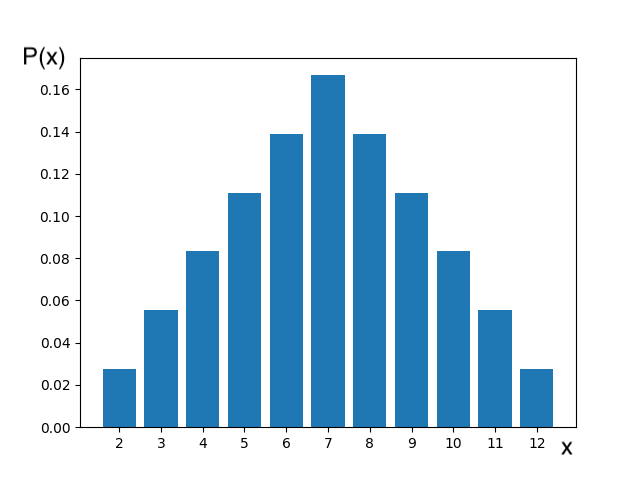
\includegraphics[width=0.5\textwidth]{disk_por}
			\caption{Porazdelitev meta dveh igralnih kock.}
		\end{figure}
		\item Porazdelitev zvezne spremenljivke - inteligenčni količnik (IQ)
		\begin{figure}[!ht]
			\centering
			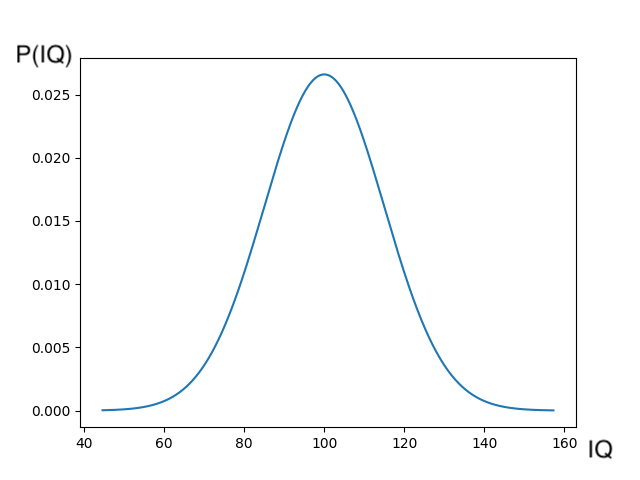
\includegraphics[width=0.5\textwidth]{iq}
			\caption{Porazdelitev IQ v populaciji ljudi.}
		\end{figure}
	\end{enumerate}
\end{zgled}

Vse možne izide porazdelitve in pogostost izidov nam predstavi funkcija verjetnosti za diskretne spremenljivke oziroma funkcija gostote verjetnosti za zvezne spremenljivke. Navedimo natančnejši definiciji:

\begin{definicija}
	\leavevmode
	\begin{itemize}
		\item \textbf{Funkcija gostote verjetnosti} (ali samo gostota verjetnosti, angl. probability density function) zvezne slučajne spremenljivke $X$ je funkcija $f: \mathbb{R} \rightarrow \mathbb{R^+}$, tako da za vsaki realni števili $a \leq b$ velja:
		\begin{equation}
			P(a \leq X \leq b) = \int_a^b f(x) \ dx.
		\end{equation}
		Drugače povedano, ploščina gostote verjetnosti med $a$ in $b$ nam pove, kakšna je verjetnost, da se zgodijo dogodki med $a$ in $b$. Veljati mora še $f(x) \geq 0$ za vse $x$ in $\int_{-\infty}^\infty f(x) \ dx = 1$.
		\item \textbf{Funkcija verjetnosti} (angl. probability mass function) diskretne slučajne spremenljivke $X$ je funkcija $p: \mathbb{R} \rightarrow [0,1]$, definirana kot
		\begin{equation}
			p(a) = P(X = a)
		\end{equation}
		za $a \in \mathbb{R}$, tj. funkcija, ki nam pove, kakšna je verjetnost da se zgodi dogodek $a$ za vse $a$. Veljati mora še $\sum_i p(a_i) = 1$, ko $i$ preteče vse možnosti.
	\end{itemize}
\end{definicija}

S tem, ko poznamo funkcijo verjetnosti oz. gostoto verjetnosti, poznamo tudi porazdelitev slučajne spremenljivke.

Poglejmo si še nekaj porazdelitev zveznih spremenljivk.

\begin{zgled}
	\leavevmode
\begin{enumerate}
	\item {
		Ena izmed osnovnih porazdelitev je \textbf{uniformna porazdelitev}. Gostota verjetnosti te porazdelitve na intervalu $[a, b]$ je definirana kot:
		\begin{equation}
			p(x) = 
			\begin{cases}
				\frac{1}{\mid b-a \mid}&, \quad x \in [a, b] \\ 
				\quad 0&, \quad sicer
			\end{cases}
		\end{equation}
	\begin{figure}[!ht]
		\centering
		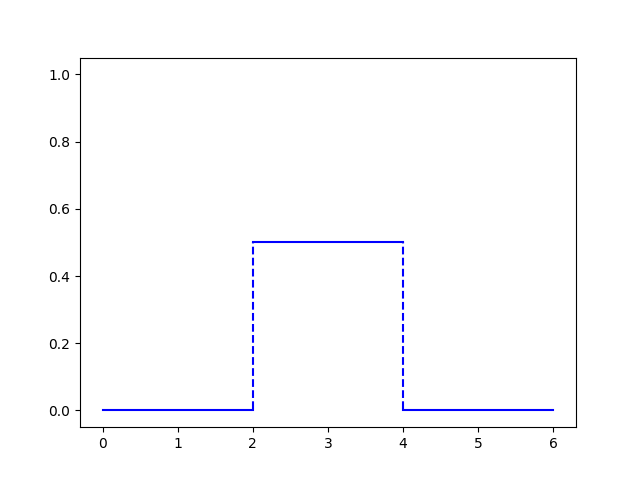
\includegraphics[width=0.45\textwidth]{uniformna}
		\caption{Uniformna porazdelitev na intervalu $[2, 4]$.}
	\end{figure}
		}
	\item {
		Zgoraj smo se že srečali s porazdelitvijo inteligenčnega količnika. To porazdelitev imenujemo \textbf{normalna} (ali \textbf{Gaussova}) \textbf{porazdelitev}, njena gostota verjetnosti pa je funkcija:
		\begin{equation}
			\N^{\mu, \sigma}(x) = \frac{1}{\sqrt{2\pi\sigma^2}}\cdot e^{-\frac{(x-\mu)^2}{2\sigma^2}},
		\end{equation}
		kjer je $\mu$ srednja vrednost (vrednost, kjer ima normalna porazdelitev maksimum - pri inteligenčnem količniku je $100$), $\sigma$ pa standardni odklon statistične populacije:
		\begin{equation}
			\sigma = \sqrt{\frac{\sum_{i=1}^N (x_i - \overset{\_}{x})^2}{N}},
		\end{equation}
		kjer je $x_i$ i-ta spremenljivka populacije, $\overset{\_}{x}$ povprečje populacije in $N$ velikost populacije (pri inteligenčnem količniku je $\sigma = 15$). Omenimo še pojem variance. \textbf{Varianca} je kvadrat standardnega odklona: $\sigma^2$.
	}
	\item {
		Kot zadnji primer si oglejmo porazdelitev \textbf{Gaussovske mešanice}. Gostota te porazdelitve je podana kot:
		\begin{equation}
			p(x) = \sum_{i=1}^n n(i) \cdot \N_i^{\mu_i, \sigma_i}(x),
		\end{equation}
		kjer so $\N_i^{\mu_i, \sigma_i}$ normalne porazdelitve, $n(i)$ pa taka pozitivna realna števila med $0$ in $1$, da velja: $\sum_{i=1}^n n(i) = 1$. Poglejmo si konkreten primer:
		\begin{equation}\label{gaussian-mixture-model}
			p(x) = \frac{1}{3} \cdot (\N^{-7,1}(x) + \N^{0,2}(x) + \N^{10,3}(x)).
		\end{equation}
		\begin{figure}[!ht]
			\centering
			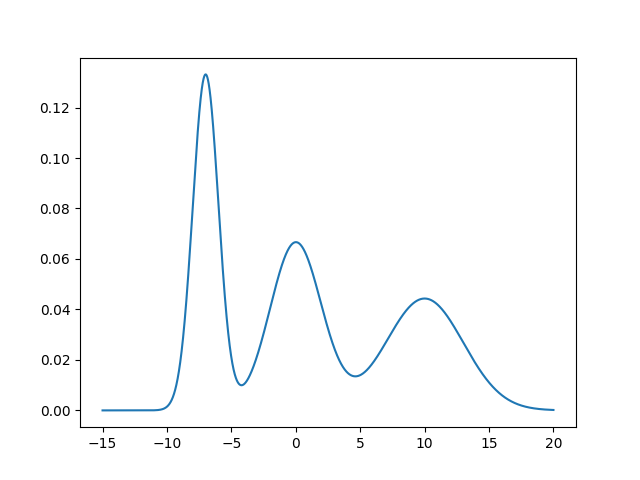
\includegraphics[width=0.5\textwidth]{gauss-mixture}
			\caption{Porazdelitev Gaussovske mešanice \eqref{gaussian-mixture-model}}
		\end{figure}
	}
\end{enumerate}
\end{zgled}
	

Za zaključek pregleda osnovnih pojmov omenimo še, da bomo v nadaljevanju velikokrat govorili o porazdelitvi in v mislih imeli gostoto verjetnosti te porazdelitve.